\documentclass[12pt,a4paper]{article}

% load packages
\usepackage{xcolor}
\usepackage{graphicx}
\usepackage{amsmath}
\usepackage{amsfonts}
\usepackage{amssymb}
\usepackage{listings}
\usepackage{hyperref}
\usepackage{algorithm}
\usepackage{algpseudocode}
\usepackage{float}
\usepackage{tabularx}
\usepackage{multirow}
\usepackage{booktabs}
\usepackage{setspace}
\setstretch{1.25}
\usepackage{appendix}
\usepackage[left=2cm,right=2cm,top=2cm,bottom=2cm]{geometry}

% set code style
\definecolor{codegreen}{rgb}{0,0.6,0}
\definecolor{codegray}{rgb}{0.5,0.5,0.5}
\definecolor{codepurple}{rgb}{0.58,0,0.82}
\definecolor{backcolour}{rgb}{0.95,0.95,0.92}


\title{Project 4 Report for Probelm 4.1}
\author{Zhu Liang}
\date{\today}

\begin{document}

\maketitle

\section{Project Description}
The primary objective of this project is the implementation of the parallel Strassen algorithm for matrix multiplication across three levels (1, 2, and 3), focusing on minimizing memory usage and communication costs.

Our approach utilizes a hierarchical multi master-slave tree (or leader-worker tree) structure. 
Each layer comprises a single leader and seven workers, where workers can serve as leaders for the subsequent layer, 
 facilitating the next level of the Strassen algorithm. 
This design allows the leader to distribute specific submatrices to its workers, 
 who later return their computed results. 
By limiting data exchange to only necessary data between leaders and workers, 
 our implementation effectively reduces communication overhead and optimizes memory consumption.


\section{Algorithm Description}
The parallel Strassen algorithm employs a divide-and-conquer approach to decompose matrix multiplication into smaller, manageable subproblems. 
These subproblems are distributed across multiple processors for parallel computation. After processing, the results are aggregated and synthesized into the final product. This recursive method continues until the subproblems reach a size conducive to sequential computation.
 
Our MPI-based implementation is a three-step process within a master-slave tree structure:
\begin{enumerate}
\item Distribute submatrices to worker processors, descending to the targeted level.
\item Perform matrix multiplication at each worker processor on the targeted level.
\item Relay results back up to the leader processor for aggregation, culminating at the \textit{root}.
\end{enumerate}
 
The following details the pseudocode for our implementation, 
beginning with an overview of the algorithm, followed by the data distribution and result collection functions.

 
\begin{algorithm}[htbp]
    \caption{Strassen Multiply Parallel}
    \label{alg:strassen_multiply_parallel}
    \begin{algorithmic}[1]
    \Procedure{StrassenMultiplyParallel}{$A, B, N, max\_level$}

        \For{$level \gets 1$ \textbf{to} $max\_level$}
            \State \Call{DistributeData}{$level$, $rank$}  
        \EndFor
        
        \State Perform matrix multiplication on all workers.
        
        \For{$level \gets max\_level$ \textbf{down to} $1$}
            \State \Call{CollectResults}{$level$, $rank$}
        \EndFor
        
        \State \Return final result on \textit{ROOT}
    \EndProcedure
    \end{algorithmic}
\end{algorithm}

\subsection{Data Distribution}
The \texttt{distribute\_data} function assigns submatrices to worker processors. This process starts at the \textit{root} processor and continues recursively to the target level. The leader processor generates pairs of submatrices ($M^A_i$ and $M^B_i$) and distributes them to its workers. The submatrices are defined as follows:

\begin{table}[htbp]
    \centering
    \begin{tabular}{cccc}
        \toprule
        $M^A_i$ & $M^B_i$ & $M_i$ & Assignment \\
        \midrule
        $M^A_1 = (A_{11} + A_{22})$ & $M^B_1 = (B_{11} + B_{22})$ & $M_1 = M^A_1 \times M^B_1$ & $\rightarrow$ Worker 1 \\
        $M^A_2 = (A_{21} + A_{22})$ & $M^B_2 = B_{11}$ & $M_2 = M^A_2 \times M^B_2$ & $\rightarrow$ Worker 2 \\
        $M^A_3 = A_{11}$ & $M^B_3 = (B_{12} - B_{22})$ & $M_3 = M^A_3 \times M^B_3$ & $\rightarrow$ Worker 3 \\
        $M^A_4 = A_{22}$ & $M^B_4 = (B_{21} - B_{11})$ & $M_4 = M^A_4 \times M^B_4$ & $\rightarrow$ Worker 4 \\
        $M^A_5 = (A_{11} + A_{12})$ & $M^B_5 = B_{22}$ & $M_5 = M^A_5 \times M^B_5$ & $\rightarrow$ Worker 5 \\
        $M^A_6 = (A_{21} - A_{11})$ & $M^B_6 = (B_{11} + B_{12})$ & $M_6 = M^A_6 \times M^B_6$ & $\rightarrow$ Worker 6 \\
        $M^A_7 = (A_{12} - A_{22})$ & $M^B_7 = (B_{21} + B_{22})$ & $M_7 = M^A_7 \times M^B_7$ & $\rightarrow$ Worker 7 \\
        \bottomrule
    \end{tabular}
    \caption{Submatrices Distributed to Each Worker}
    \label{tab:submatrices}
\end{table}


All $M^A_i$ and $M^B_i$ submatrices are of the same size and are sent to seven cores for computation. The generation and calculation of each $M^A_i$ and $M^B_i$ occur at the leader core. 
This approach ensures uniformity in the format of the distributed data and facilitates further distribution. 
Although it leads to a non-parallel computation of certain addition and subtraction operations, 
these operations are computationally less intensive compared to multiplication. Hence, we believe the benefits outweigh the costs.

% pesudo code
\begin{algorithm}[htbp]
    \caption{Distribute Data}
    \label{alg:distribute_data}
    \begin{algorithmic}[1]
    \Procedure{DistributeData}{$level$, $rank$}
        \If{$rank$ is leader under $level$}
            \State Send all $M^A_i, M^B_i$ to its worker $i$
        \EndIf
        
        \If{$rank$ is worker under $level$}
            \State Receive $M^A_i, M^B_i$ from its leader
       \EndIf
    \EndProcedure
    \end{algorithmic}
\end{algorithm}


\subsection{Result Collection}
The \texttt{collect\_results} function is responsible for gathering computation outcomes from worker processors and assimilating them into a unified matrix. This reverse hierarchical procedure commences at the designated target level and ascends to the \textit{root} processor. Each leader processor acquires partial results ($M_1$ to $M_7$) from its subordinates and integrates them to construct the final matrix. The integration is delineated as follows:

\begin{table}[htbp]
\centering
\begin{tabular}{ccl}
\toprule
\textbf{Submatrix} & \textbf{Aggregated Components} \\
\midrule
$C_{11}$ & $M_1 + M_4 - M_5 + M_7$ \\
$C_{12}$ & $M_3 + M_5$ \\
$C_{21}$ & $M_2 + M_4$ \\
$C_{22}$ & $M_1 - M_2 + M_3 + M_6$ \\
\bottomrule
\end{tabular}
\caption{Aggregation of Results from Worker Processors}
\label{tab:aggregation}
\end{table}

This table succinctly illustrates the process of assembling the final matrix from the individual components calculated by the workers.

% pesudo code
\begin{algorithm}[htbp]
    \caption{Collect Results}
    \label{alg:collect_results}
    \begin{algorithmic}[1]
    \Procedure{CollectResults}{$level$, $rank$}
        \If{$rank$ is leader under $level$}
            \State Receive all $M_i$ from its workers
            \State Aggregate $M_i$ to $C$
        \EndIf
        
        \If{$rank$ is worker under $level$}
            \State Send $M_i$ to its leader
       \EndIf
    \EndProcedure
    \end{algorithmic}
\end{algorithm}   


As outlined in Algorithms \ref{alg:distribute_data} and \ref{alg:collect_results}, establishing the leader-worker relationships for each processor at different levels is crucial. 
This is achieved through a recursive tree structure, where the relationships are dictated by the processors' ranks. 
These relationships remain consistent across all levels. 
For an in-depth understanding of this tree structure, please refer to the Appendix \ref{appendix:tree_structure}.

This description is intentionally streamlined, 
omitting many details and supporting functions for brevity. 
More details can be gleaned from the source code file \texttt{functions.c}.

\section{Results}
\subsection{Performance}
Notice that the level 1, 2, 3 of the parallel Strassen algorithm requires 7, 49, 343 processors respectively to 
fully utilize the parallelism. We will run the parallel Strassen algorithm with 7, 49, 343 processors respectively.
\begin{table}[ht]
    \centering
    \begin{tabular}{cccc}
        \toprule
        & \multicolumn{3}{c}{Parallel Strassen Algorithm} \\
        \cmidrule(lr){2-4}
        (in seconds) &  level 1  &  level 2  &  level 3 \\
        & (cores = 7) & (cores = 49) & (cores = 343) \\
        \midrule
        \( N = 2^8 \)  & 0.029430 & 0.010317 & 0.040137 \\
        \( N = 2^{10} \) & 1.757423 & 0.284435 & 0.274502 \\
        \( N = 2^{12} \) & 63.811983 & 9.049598 & 2.902417 \\
        \bottomrule
    \end{tabular}
    \caption{Performance of the Parallel Strassen Algorithm at different levels.}
    \label{tab:results}
\end{table}


\subsection{Speedup}
Speedup is a metric that quantifies the performance improvement of a parallel algorithm compared to its sequential counterpart. 
The orginal speedup \( S \) for \( P \) processors for size $N$ problem is defined as:

\begin{equation*}
    S(P, N) = \frac{T(1,N)}{T(P, N)}
\end{equation*}

where \( T(1,N) \) is the execution time of the sequential algorithm and 
 \( T(P, N) \) is the execution time of the parallel algorithm using \( P \) processors.

However, in our case, the sequential algorithm on single core is not implemented. Instead, 
 we use the performance of the parallel algorithm with \( P = 7 \) as the baseline.
The updated speedup \( S \) is defined as:

\begin{equation}
    \label{eqn:updated_speedup}
    S(P, N) = 7 \times \frac{T(7,N)}{T(P, N)}
\end{equation}


 Using the data from Table \ref{tab:results}, 
  we can compute the speedup for matrix multiplication for different 
  matrix sizes \( N \) and varying number of processors \( P \) (under level 1, 2, 3). 
Since the baseline is the performance of the parallel algorithm with \( P = 7 \), 
 the speedup values are computed using Equation \ref{eqn:updated_speedup}.
The speedup values for each \( N \) (under level 2 and level 3) are plotted in the following Figure \ref{fig:speedup_curve}.

\begin{figure}
    \centering
    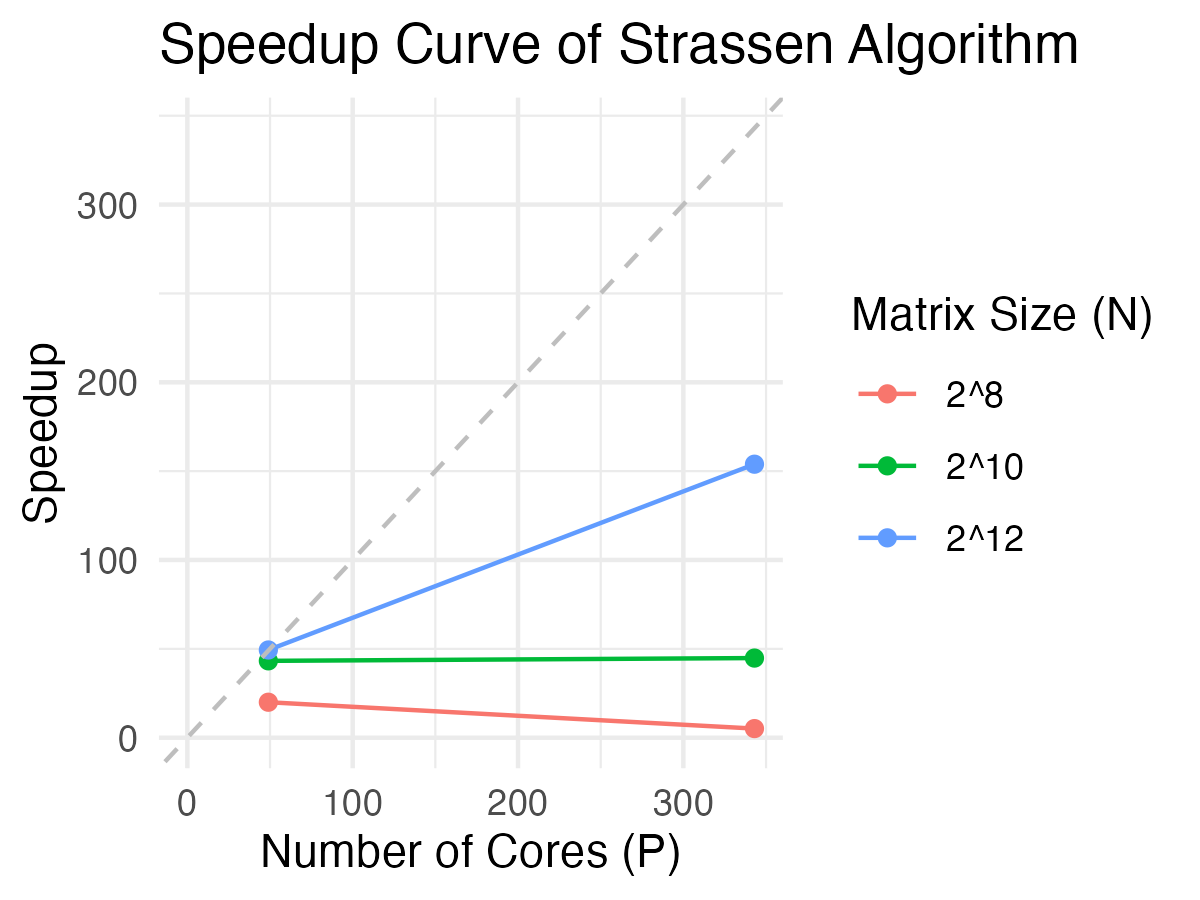
\includegraphics[width=0.6\textwidth]{speedup_curve.png}
    \caption{Speedup Curve for Matrix Sizes \( N \)}
    \label{fig:speedup_curve}
\end{figure}

\section{Analysis}
The speedup curve, as shown in Figure \ref{fig:speedup_curve}, demonstrates the scalability of our parallel Strassen algorithm with varying numbers of processors. An ideal linear speedup is indicated by a dashed line, while the solid lines represent the actual speedup for different matrix sizes. The observed trends can be summarized as follows:

For \(N = 2^8\), the speedup decreases with additional processors, suggesting that the overhead of communication dominates the benefits of parallel computation due to the small size of the matrices. 

When \(N = 2^{10}\), the speedup curve plateaus, indicating that the computational load and communication overhead reach a balance. 

For \(N = 2^{12}\), there is a noticeable increase in speedup, implying that the computation benefits substantially from parallel execution.

The underlying causes for these trends can be attributed to two main factors:

\begin{itemize}
    \item \textbf{Communication Overhead:} As the number of processors increases, the communication overhead can become a bottleneck, especially for smaller matrices where the communication cost outweighs the computation time.
    \item \textbf{Computation to Communication Ratio:} For larger matrices, the computation to communication ratio improves, allowing the algorithm to better exploit the parallel architecture. This results in a higher speedup as the computation workload per processor increases, which is more pronounced for \(N = 2^{12}\).
\end{itemize}

This analysis highlights the critical balance between computation and communication in parallel algorithms and will guide our efforts in optimization, focusing on minimizing communication costs and improving load distribution among processors.

\appendix
% print Appendix
\clearpage
\section{Tree Structure for Leader-Worker Relationships}
\label{appendix:tree_structure}

The leader-worker relationships within the parallel Strassen algorithm are organized in a hierarchical tree structure. This structure is pivotal for determining the flow of data distribution and result collection across different levels of computation. The tree structure is recursive, with each leader processor being connected to a set of worker processors. The following table illustrates these relationships:

\begin{table}[htbp]
    \centering
    \begin{tabular}{cl}
        \toprule
        \textbf{Leader Rank} & \textbf{Worker Ranks} \\
        \midrule
        0 & [0, 1, 2, 3, 4, 5, 6] \\
        1 & [7, 8, 9, 10, 11, 12, 13] \\
        2 & [14, 15, 16, 17, 18, 19, 20] \\
        3 & [21, 22, 23, 24, 25, 26, 27] \\
        4 & [28, 29, 30, 31, 32, 33, 34] \\
        5 & [35, 36, 37, 38, 39, 40, 41] \\
        6 & [42, 43, 44, 45, 46, 47, 48] \\
        % Continue as needed...
        % print and so on on the next line 
        ... & ... \\
        \bottomrule
    \end{tabular}
    \caption{Leader to Worker Relationships in the Tree Structure}
    \label{tab:leader_worker_relationships}
\end{table}

Each processor's rank in the tree structure determines its specific role, ensuring consistent leader-worker assignments throughout the parallel computation of the Strassen algorithm. This design reuses leaders from one level as workers in the subsequent level, facilitating the implementation of levels 1, 2, and 3 with 7, 49, and 343 processors, respectively. The hierarchy is pre-established and remains unchanged throughout the process.

To identify the leader and worker ranks at any given level, we employ the \texttt{get\_leade\_rank} and \texttt{get\_worker\_rank} functions. Additionally, the functions \texttt{is\_leader} and \texttt{is\_worker} determine whether a processor serves as a leader or a worker at a particular level. For a detailed understanding of these functionalities, please refer to the \texttt{functions.c} file in the source code.

\subsection{Special Case: \textit{root}}
\label{subsec:special_case_root}
As evident from the leader-worker relationships detailed in , the \textit{root} processor (rank 0) 
 uniquely acts as both sender and receiver simultaneously. 
 This dual role could lead to deadlock situations when employing standard MPI communication methods like \texttt{MPI\_Isend} and \texttt{MPI\_Irecv}.

To circumvent this issue, a special handling mechanism is implemented specifically for the \textit{root} processor. Instead of using MPI functions for sending and receiving data, the \textit{root} processor directly writes the relevant submatrices into its memory buffer and later reads from this buffer for further processing. This approach not only prevents deadlock scenarios but also reduces communication overhead, as it eliminates the need for additional message-passing tasks for the \textit{root} processor. By directly manipulating the memory, we maintain the efficiency and fluidity of the algorithm's execution, especially at the top level of the tree structure.





\section*{File Notes}
The source code of the program is in the \texttt{project4} folder. 
For more details, please refer to the \texttt{README.md} file in the folder.

\end{document}


